\subsection{UML2-Komponentendiagramm}

    \begin{figure}[H]
        \centering
        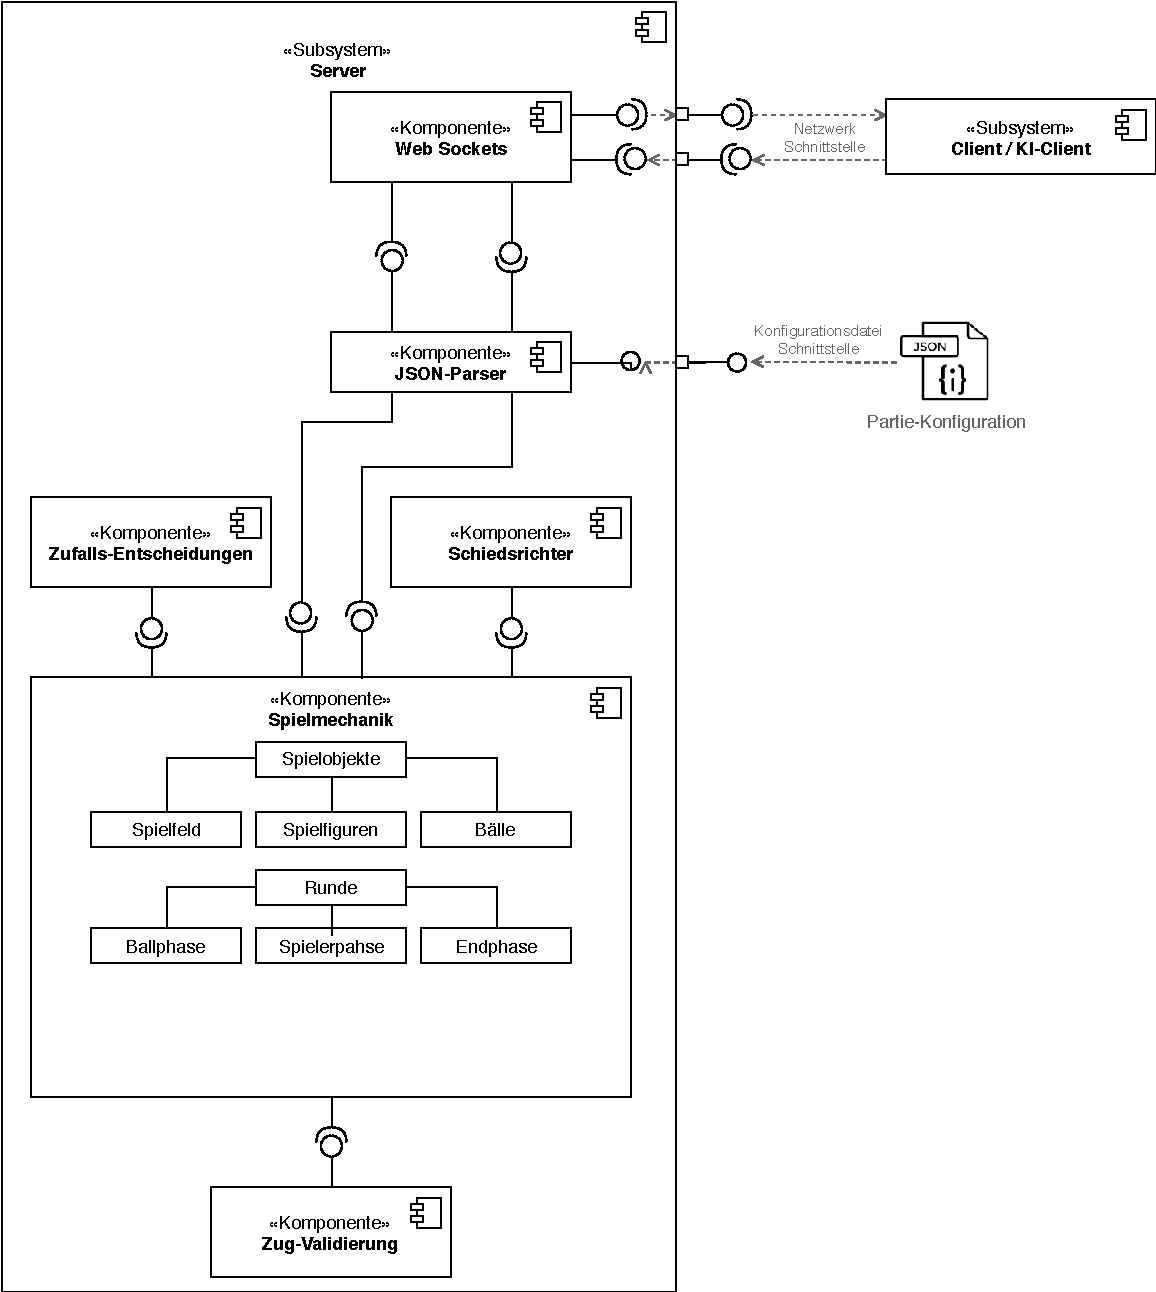
\includegraphics[scale=0.75]{images/Server-Architektur_DrawIO-Gesammt.pdf}
    \end{figure}

\subsection{Beschreibungen}

    \begin{description}
        
        \item[Server]
        Beim Subsystem Server handelt es sich um die Konsolenanwendung, die als Schnittstelle für zwei oder mehr Clients dient. Die Serveranwendung kümmert sich dabei primär um die Spielsteuerung und agiert dabei unabhängig von den Client-Anwendungen.
        
        \item[Spielmechanik]
        Die Spielmechanik ist die zentrale Komponente des Server Subsystems. Diese bildet dabei die komplette Partie intern ab. In der Spielmechanik sind also zu jeder Zeit die aktuellsten Status der Spielobjekte hinterlegt. Während eines Spiels senden die Clients ihre gewünschten Züge an den Server. Die Spielmechanik wertet die Züge, nachdem sie validiert und vom Schiedsrichter geprüft wurden, aus und aktualisiert dann gegebenenfalls die aktuelle Spielsituation. Diese wird im Anschluss wieder vom Server aus zu den einzelnen Clients ausgegeben. Als zentrale Komponente des Server Subsystems ist es zwingend notwendig, dass diese Komponente als Einheit gesehen wird, da ohne diesen Teil kein das Spielen nicht möglich wäre.
        
        \item[Zug-Validierung]
        Die Zug-Validierung prüft, ob die Züge, die von einem Spieler über seinen Client übermittelt werden, grundsätzlich möglich sind. Dabei wird jedoch nicht geprüft ob der gewünschte Zug ein Foul darstellt. Notwendig ist diese Prüfung, da nicht sichergestellt ist, dass jede Client-Anwendung tatsächlich prüft ob die Züge die ein Spieler tätigen will auch grundsätzlich möglich sind. Die Komponente ist aus der eigentlichen Spielmechanik ausgegliedert, da die Zug-Validierung auch in anderen Subsystem eingesetzt werden könnte, z.b. einer Client-Anwendung.			
        
        \item[Schiedsrichter]
        Die Schiedsrichter Komponente des Server Subsystems. Möchte ein Spieler einen verbotenen Zug tätigen, wird in der Schiedsrichter Komponente die Entscheidung getroffen, ob der Spieler bestraft wird. Diese Komponente ist aus der Spielmechanik ausgegliedert, da da das Spiel grundsätzlich auch ohne diese Komponente möglich ist und daher diese Komponente in einem nachgelagerten Entwicklungsschritt implementiert werden kann.
        
        \item[Zufalls-Entscheidungen]
        Dies Komponente stellt der Spielmechanik und der Schiedsrichter Komponente eine Schnittstelle zur Verfügung, die es erlaubt die vielen Zufalls-Ereignisse in einer Partie auszuwerten.
        
        \item[Kommunikator]
        Der Kommunikator bildet die Komponente, die sich um die Datenübertragung zwischen der Server- und den Client-Anwendungen kümmert. Dabei werden dort zum einen die Status der Verbindungen zu den Clients überwacht und verwaltet. Zum anderen wir die Datenübertragung in beide Richtungen bereitgestellt. Da auch in den Client-Anwendungen eine ähnliche Komponente von Nöten ist, bietet es sich an, diese Funktionalitäten in einer eigenen Komponente auszulagern.
        
        \item[JSON-Parser]
        Der JSON-Parser (de-) serialisiert die Objekte der Spiellogik. Da auch in den Client-Anwendungen eine ähnliche Komponente von Nöten ist, bietet es sich an, diese Funktionalitäten in einer eigenen Komponente auszulagern.  

    \end{description}
    
\subsection{Zuordnung der Funktionalen Anforderungen}

Die funktionalen Anforderungen gemäß dem Pflichtenheft werden den Komponenten folgendermaßen zugeteilt:

\begin{table}[h]
\centering
\begin{tabular}{|l|l|}
    \hline
    \textbf{Komponente} & \textbf{Abgedeckte funktionale Anforderungen}\\ \hline
    Spielmechanik & FA1 - FA36 \\
    & FA43 - FA52 \\
    & FA56 \\
    & FA59 \\ \hline
    
    Schiedsrichter & FA36 - FA42 \\ \hline
    
    Zug-Validierung & FA67 \\ \hline
    
    Zufalls-Entscheidungen & FA58 \\ \hline	
    
    Kommunikator & FA55 \\ \hline
    
    JSON-Konverter & FA53 \\
    & FA57\\ \hline


\end{tabular}
\end{table}
